\documentclass[12pt,a4paper]{report}

\usepackage[utf8]{inputenc}
\usepackage[T1]{fontenc}
\usepackage[french]{babel}
\usepackage{geometry}
\usepackage{graphicx}
\usepackage[table]{xcolor}
\usepackage{array}
\usepackage{booktabs}
\usepackage{longtable}
\usepackage{float}
\usepackage{caption}
\usepackage{hyperref}
\usepackage{titlesec}
\usepackage{setspace}
\usepackage{enumitem}
\usepackage{fancyhdr}
\usepackage{tikz}

\geometry{top=2.4cm,bottom=2.4cm,left=2.6cm,right=2.6cm}
\onehalfspacing
\setlength{\parindent}{0.8cm}
\setlength{\parskip}{0.35em}

\definecolor{TitleColor}{HTML}{3B2F2F}
\definecolor{AccentColor}{HTML}{5C6B3C}
\definecolor{LightBox}{HTML}{F4F1EA}
\definecolor{TableHead}{HTML}{E8E3D8}
\definecolor{RuleColor}{HTML}{7A6A53}

\hypersetup{
  colorlinks=true,
  linkcolor=TitleColor,
  urlcolor=AccentColor,
  citecolor=TitleColor
}

\titleformat{\chapter}
  {\normalfont\huge\bfseries\color{TitleColor}}
  {\thechapter.}{0.7em}{}
\titleformat{\section}
  {\normalfont\Large\bfseries\color{TitleColor}}
  {\thesection}{0.7em}{}
\titleformat{\subsection}
  {\normalfont\large\bfseries\color{AccentColor}}
  {\thesubsection}{0.7em}{}

\pagestyle{fancy}
\fancyhf{}
\lhead{Gestion des accès et présence à domicile}
\rhead{\thepage}
\renewcommand{\headrulewidth}{0.4pt}

\newcommand{\placeholder}[2]{
  \begin{center}
    \fcolorbox{RuleColor}{LightBox}{
      \begin{minipage}{0.86\textwidth}
        \centering
        \vspace{0.6cm}
        \textbf{#1}\\[0.25cm]
        #2
        \vspace{0.6cm}
      \end{minipage}
    }
  \end{center}
}

\begin{document}

\begin{titlepage}
  \centering
  \vspace*{0.4cm}

  \fcolorbox{RuleColor}{LightBox}{
    \begin{minipage}{0.36\textwidth}
      \centering
      \vspace{1.2cm}
      \textbf{Logo de l'université}\\
      \small Placeholder image
      \vspace{1.2cm}
    \end{minipage}
  }

  \vspace{0.8cm}
  {\Large \textbf{Université : [Nom de l'université]}}\\[0.2cm]
  {\large Filière : Master GLCC - Informatique}\\
  {\large Module : Systèmes embarqués et IoT}\\
  {\large Année d'étude : [Année universitaire]}\\[1.1cm]

  {\large Projet IoT - ESP32 + Wokwi + Blynk}\\[0.4cm]
  {\Huge \textbf{Système de gestion des accès et présence à domicile}}\\[0.35cm]
  {\Large Mini-rapport de synthèse}\\[1.2cm]

  \begin{tabular}{>{\bfseries}p{5.2cm}p{8.2cm}}
    Réalisé par & Étudiant 1 : [Nom et prénom] \\
                 & Étudiant 2 : [Nom et prénom] \\
                 & Étudiant 3 : [Nom et prénom] \\[0.2cm]
    Encadré par & Professeur : [Nom du professeur] \\[0.2cm]
    Microcontrôleur & ESP32 DevKit C v4 \\
    Supervision & Blynk avec Wi-Fi simulé Wokwi-GUEST \\
    Environnement & Simulation Wokwi et développement Arduino C/C++ \\
  \end{tabular}

  \vfill
  {\large Année universitaire : 2025--2026}
\end{titlepage}

\pagenumbering{roman}
\tableofcontents
\clearpage
\listoffigures
\clearpage

\chapter*{Table des mots-clés}
\addcontentsline{toc}{chapter}{Table des mots-clés}
\begin{table}[H]
  \centering
  \caption{Mots-clés du projet}
  \begin{tabular}{p{4cm}p{10cm}}
    \toprule
    \rowcolor{TableHead}
    \textbf{Mot-clé} & \textbf{Description} \\
    \midrule
    IoT & Réseau d'objets connectés permettant la collecte, le traitement et la supervision de données à distance. \\
    ESP32 & Microcontrôleur principal utilisé pour lire les capteurs, exécuter la logique et communiquer avec Blynk. \\
    Wokwi & Plateforme de simulation utilisée pour tester le montage et le code avant la réalisation matérielle. \\
    Blynk & Plateforme de supervision IoT utilisée pour afficher l'état du logement et envoyer des notifications. \\
    Fusion de capteurs & Combinaison du PIR et du HC-SR04 afin de confirmer la présence avec plus de fiabilité. \\
    Présence & État validé lorsque le mouvement est détecté et qu'une distance inférieure à 200 cm est mesurée. \\
    Absence prolongée & Situation où aucune présence n'est confirmée pendant une durée importante, avec possibilité d'alerte. \\
    \bottomrule
  \end{tabular}
\end{table}

\clearpage
\pagenumbering{arabic}

\chapter*{Introduction}
\addcontentsline{toc}{chapter}{Introduction}
Le développement des systèmes domotiques a rendu possible la surveillance intelligente d'un logement à partir de composants simples, économiques et faciles à programmer. Dans ce contexte, le projet présenté dans ce rapport consiste à concevoir un système IoT capable de gérer les accès et la présence à domicile. L'objectif n'est pas seulement de détecter un mouvement, mais de proposer une chaîne complète allant de l'acquisition des données par les capteurs jusqu'à l'affichage local et la supervision à distance.

Le système repose sur un ESP32 DevKit C v4 programmé avec l'environnement Arduino C/C++. Il exploite un capteur PIR pour détecter le mouvement, un capteur ultrason HC-SR04 pour confirmer la proximité, un DHT22 pour mesurer la température, un bouton poussoir pour simuler une sonnette, un afficheur LCD I2C, deux LEDs et un buzzer. La supervision est assurée par Blynk, tandis que la validation initiale du montage est réalisée avec Wokwi. Cette organisation permet de tester les fonctions principales sans dépendre immédiatement d'un prototype physique.

La portée du projet couvre la détection de présence, la distinction entre un logement vide et occupé, la gestion d'un événement visiteur, l'affichage de l'état courant et l'envoi d'informations vers une interface distante. Le projet introduit également la notion d'absence prolongée, qui peut devenir importante lorsque la température intérieure est basse. Cette situation peut signaler un risque pour le logement ou indiquer qu'une surveillance renforcée est nécessaire.

Une partie importante du travail concerne la fiabilité de la décision. Un capteur PIR seul peut produire des détections non désirées, tandis qu'une mesure de distance seule ne prouve pas qu'une personne est réellement présente. Pour cette raison, le système applique une fusion de capteurs : la présence est confirmée uniquement lorsque le PIR est actif et que le HC-SR04 mesure une distance inférieure à 200 cm. Cette règle rend le comportement plus robuste et montre que le projet ne se limite pas à une lecture isolée de capteurs, mais met en place une logique embarquée cohérente.

\chapter{Analyse du besoin}
Le besoin principal est de disposer d'un système capable d'informer l'utilisateur sur l'état d'occupation d'un logement. Dans une situation réelle, l'utilisateur peut vouloir savoir si une personne est présente, si un visiteur s'est présenté à la porte ou si une absence devient anormalement longue. Ces informations peuvent améliorer la sécurité, le confort et la réactivité de l'utilisateur face à certains événements.

Le système doit rester simple à comprendre et à démontrer. Il doit donc afficher localement les informations importantes grâce au LCD, aux LEDs et au buzzer. En parallèle, il doit transmettre les données principales vers Blynk afin que l'utilisateur puisse consulter l'état du logement à distance. La combinaison entre retour local et supervision distante constitue un point essentiel du projet, car elle rapproche la simulation d'un cas d'utilisation réel.

\section{Objectifs fonctionnels}
Les objectifs fonctionnels retenus sont les suivants :
\begin{itemize}[leftmargin=1.3cm]
  \item détecter une présence probable dans le logement ;
  \item limiter les faux positifs grâce à la fusion du PIR et du capteur ultrason ;
  \item signaler un visiteur lorsque le bouton de sonnette est activé ;
  \item afficher localement l'état courant sur un écran LCD I2C ;
  \item activer des sorties visuelles et sonores selon les événements ;
  \item transmettre les mesures et les états vers Blynk ;
  \item prévoir une alerte en cas d'absence prolongée et de température basse.
\end{itemize}

\section{Contraintes du projet}
Le projet doit être réalisable dans un environnement pédagogique. La simulation Wokwi permet de vérifier rapidement le montage, mais elle impose aussi certaines adaptations. Par exemple, les délais réels de plusieurs minutes peuvent être raccourcis pendant la démonstration pour éviter une attente trop longue. Cette adaptation doit être clairement mentionnée dans le code et dans le rapport afin de ne pas confondre la logique réelle avec la logique de test.

\chapter{Architecture générale}
L'architecture du système est organisée en quatre parties : acquisition, traitement, sorties locales et supervision IoT. Cette séparation facilite la lecture du projet, car chaque bloc a un rôle bien défini. Les capteurs collectent les informations du logement, l'ESP32 prend les décisions, les sorties locales informent les personnes présentes et Blynk assure la consultation à distance.

\begin{figure}[H]
  \centering
  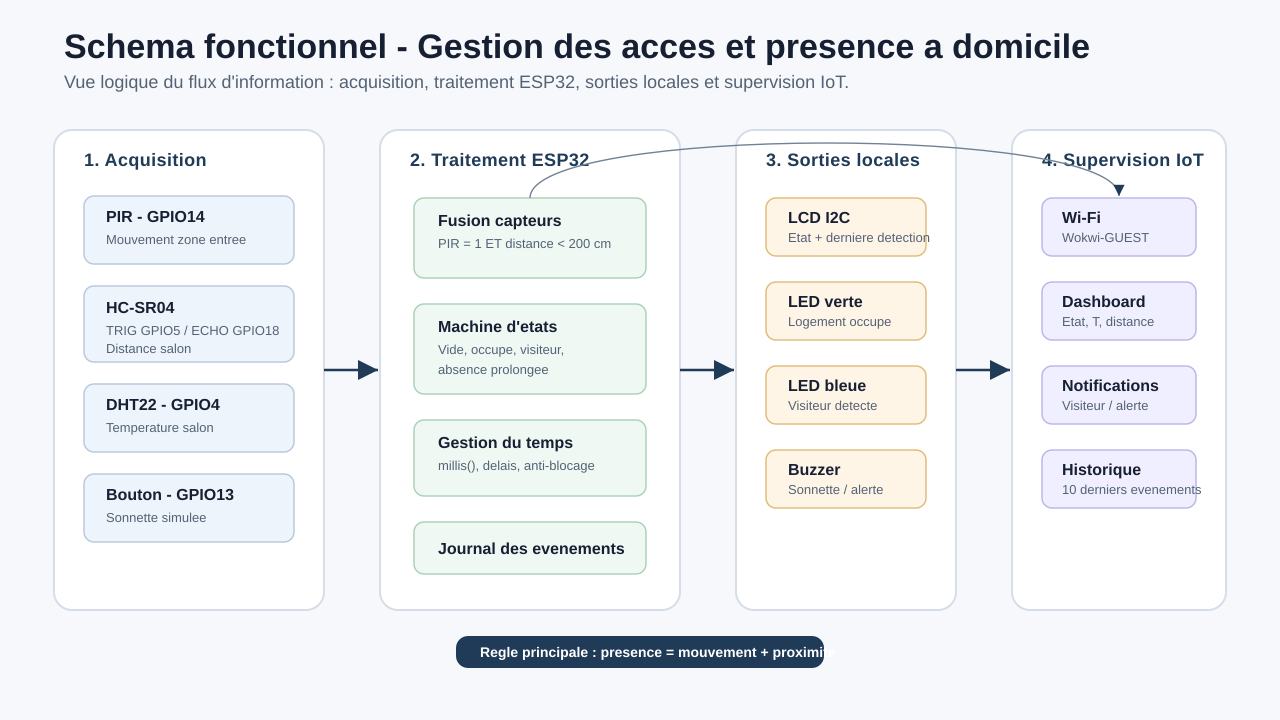
\includegraphics[width=0.95\textwidth]{assets/schema_fonctionnel.png}
  \caption{Schéma fonctionnel du système}
  \label{fig:schema-fonctionnel}
\end{figure}

Le flux de fonctionnement est progressif. Les capteurs envoient d'abord leurs valeurs vers l'ESP32. Ensuite, le programme applique les règles de décision, met à jour l'état du logement, commande les LEDs, le buzzer et le LCD, puis publie les informations utiles vers Blynk. Ce découpage permet aussi de tester chaque partie séparément avant de valider le comportement global.

\chapter{Choix des composants}
\begin{longtable}{p{3.5cm}p{3.6cm}p{7cm}}
  \caption{Composants utilisés dans le projet}\\
  \toprule
  \rowcolor{TableHead}
  \textbf{Composant} & \textbf{Broche ESP32} & \textbf{Rôle et justification} \\
  \midrule
  \endfirsthead
  \toprule
  \rowcolor{TableHead}
  \textbf{Composant} & \textbf{Broche ESP32} & \textbf{Rôle et justification} \\
  \midrule
  \endhead
  PIR motion sensor & GPIO14 & Détecte le mouvement dans la zone d'entrée. Il sert de premier indicateur de présence, mais sa décision est confirmée par le capteur ultrason. \\
  HC-SR04 TRIG/ECHO & GPIO5 / GPIO18 & Mesure la distance afin de vérifier qu'un objet ou une personne se trouve réellement dans la zone surveillée. \\
  DHT22 & GPIO4 & Mesure la température ambiante. Cette donnée peut être utilisée pour déclencher une alerte lors d'une absence prolongée avec température basse. \\
  Bouton poussoir & GPIO13 & Simule une sonnette. Il permet de tester facilement le scénario de visiteur dans Wokwi. \\
  LCD I2C 16x2 & GPIO21 / GPIO22 & Affiche l'état du logement et la dernière détection. Il donne un retour local compréhensible sans téléphone. \\
  LED verte & GPIO25 & Indique visuellement que le logement est occupé. \\
  LED bleue & GPIO26 & Indique un visiteur ou un événement de sonnette. \\
  Buzzer & GPIO12 & Produit un signal sonore lors de la sonnette ou d'une alerte. \\
  \bottomrule
\end{longtable}

\chapter{Fonctionnement du système}
La règle principale de décision est la suivante :
\begin{center}
  \textbf{Présence confirmée = PIR actif ET distance HC-SR04 < 200 cm}
\end{center}

Cette règle est volontairement plus stricte qu'une simple détection de mouvement. Le PIR peut réagir à des variations ou à des comportements de simulation, alors que le HC-SR04 peut mesurer un objet proche sans qu'il s'agisse d'une personne en mouvement. En exigeant les deux conditions, le système réduit les erreurs et améliore la cohérence de l'état affiché.

\begin{table}[H]
  \centering
  \caption{Matrice de décision de présence}
  \begin{tabular}{p{2cm}p{3.5cm}p{4cm}p{5cm}}
    \toprule
    \rowcolor{TableHead}
    \textbf{PIR} & \textbf{Distance} & \textbf{Décision} & \textbf{Explication} \\
    \midrule
    0 & $\geq$ 200 cm & Vide & Aucun mouvement et aucun objet proche ne sont détectés. \\
    1 & $\geq$ 200 cm & Faux positif filtré & Le mouvement seul ne suffit pas pour confirmer une présence. \\
    0 & $<$ 200 cm & Non comptabilisé & Un objet proche est détecté, mais aucun mouvement ne confirme une personne. \\
    1 & $<$ 200 cm & Présence confirmée & Les deux capteurs indiquent une situation cohérente. \\
    \bottomrule
  \end{tabular}
\end{table}

\section{États du système}
Le programme peut être représenté par quatre états principaux. L'état \textit{vide} correspond à une absence de présence confirmée. L'état \textit{occupé} est activé lorsque la règle de fusion est validée. L'état \textit{visiteur} apparaît lorsque le bouton de sonnette est pressé. Enfin, l'état \textit{absence prolongée} est déclenché lorsqu'aucune présence n'est détectée pendant une durée importante.

Cette approche par états rend le programme plus lisible. Elle évite de disperser les conditions dans toute la boucle principale et permet de relier chaque sortie à une situation claire. Elle facilite également les tests, car chaque scénario peut être vérifié séparément.

\chapter{Architecture logicielle}
Le code Arduino est structuré autour de fonctions spécialisées. Cette organisation évite de placer toute la logique dans la fonction \texttt{loop()}, ce qui rendrait le programme difficile à maintenir. Les temporisations sont gérées avec \texttt{millis()} afin de continuer à lire les capteurs pendant que le système attend un changement d'état.

\begin{table}[H]
  \centering
  \caption{Organisation logicielle proposée}
  \begin{tabular}{p{5cm}p{9cm}}
    \toprule
    \rowcolor{TableHead}
    \textbf{Fonction} & \textbf{Rôle} \\
    \midrule
    \texttt{readSensors()} & Lit le PIR, le HC-SR04, le DHT22 et le bouton de sonnette. \\
    \texttt{updatePresenceState()} & Applique la fusion de capteurs et met à jour l'état du logement. \\
    \texttt{handleDoorbell()} & Gère le visiteur, la LED bleue, le buzzer et la notification. \\
    \texttt{updateOutputs()} & Commande les LEDs, le buzzer et les sorties locales. \\
    \texttt{updateLcd()} & Affiche l'état courant et la dernière détection sur le LCD. \\
    \texttt{sendToBlynk()} & Envoie les mesures et les états vers les pins virtuels de Blynk. \\
    \bottomrule
  \end{tabular}
\end{table}

Cette structure améliore aussi la qualité du débogage. Si une sortie ne réagit pas correctement, il devient possible de vérifier séparément la lecture des capteurs, la décision logique et la commande matérielle. Elle correspond donc à une démarche de développement progressive et adaptée à un mini-projet IoT.

\chapter{Simulation Wokwi}
La simulation Wokwi constitue la première étape de validation. Elle permet de vérifier les connexions, le comportement du code et la réaction des sorties sans disposer immédiatement du matériel réel. Le fichier \texttt{diagram.json} décrit le montage, tandis que \texttt{sketch.ino} contient le programme destiné à l'ESP32.

\placeholder{Capture à insérer - Montage Wokwi}{Ajouter ici une capture du circuit Wokwi avec l'ESP32, les capteurs, le LCD, les LEDs et le buzzer.}

Les scénarios de test doivent être joués directement dans la simulation. Il est notamment important de tester le PIR seul, le HC-SR04 seul, la combinaison des deux, le bouton de sonnette et l'absence prolongée. Ces essais prouvent que la logique embarquée répond aux cas attendus.

\chapter{Intégration Blynk}
Blynk est utilisé pour transformer le prototype en système supervisable à distance. Les informations envoyées vers l'application peuvent inclure l'état du logement, la température, la distance mesurée, l'état du PIR, le dernier événement et le mode vacances. Cette interface complète les sorties locales, car elle permet à l'utilisateur de consulter le logement même s'il n'est pas devant le montage.

\begin{table}[H]
  \centering
  \caption{Datastreams Blynk proposés}
  \begin{tabular}{p{2.5cm}p{5cm}p{6.5cm}}
    \toprule
    \rowcolor{TableHead}
    \textbf{Pin virtuel} & \textbf{Donnée} & \textbf{Widget conseillé} \\
    \midrule
    V0 & État du logement & Label ou Value Display \\
    V1 & Température DHT22 & Gauge \\
    V2 & Dernier événement & Label ou Terminal \\
    V3 & Mode vacances & Switch \\
    V4 & Distance HC-SR04 & Gauge \\
    V5 & État PIR & LED ou Indicator \\
    V6 & Heures d'occupation estimées & Value Display \\
    \bottomrule
  \end{tabular}
\end{table}

\placeholder{Capture à insérer - Dashboard Blynk}{Ajouter ici une capture du tableau de bord Blynk et des notifications configurées.}

\chapter{Validation et tests}
La validation doit montrer que chaque état du système est atteint dans les bonnes conditions. Le tableau suivant regroupe les principaux scénarios. La colonne résultat peut être complétée après la démonstration ou après les captures Wokwi/Blynk.

\begin{longtable}{p{1cm}p{3.2cm}p{4.1cm}p{4.4cm}p{2.2cm}}
  \caption{Tableau de validation du système}\\
  \toprule
  \rowcolor{TableHead}
  \textbf{N} & \textbf{Scénario} & \textbf{Entrées} & \textbf{Comportement attendu} & \textbf{Résultat} \\
  \midrule
  \endfirsthead
  \toprule
  \rowcolor{TableHead}
  \textbf{N} & \textbf{Scénario} & \textbf{Entrées} & \textbf{Comportement attendu} & \textbf{Résultat} \\
  \midrule
  \endhead
  1 & PIR seul & PIR = 1, distance $\geq$ 200 cm & Présence non confirmée, pas d'état occupé. & À compléter \\
  2 & Ultrason seul & PIR = 0, distance $<$ 200 cm & Présence non confirmée, objet proche seulement. & À compléter \\
  3 & Présence confirmée & PIR = 1, distance $<$ 200 cm & État occupé, LED verte activée, LCD mis à jour. & À compléter \\
  4 & Timeout absence & Aucune détection pendant le délai & État vide après expiration du délai. & À compléter \\
  5 & Absence et froid & Absence prolongée, température $<$ 10~°C & Notification Blynk et alerte locale selon configuration. & À compléter \\
  6 & Sonnette & Bouton pressé & État visiteur, LED bleue, buzzer et notification. & À compléter \\
  7 & Mode vacances & Mode vacances actif avec mouvement & Alerte renforcée vers Blynk. & À compléter \\
  \bottomrule
\end{longtable}

\chapter{Difficultés rencontrées}
La première difficulté concerne la fiabilité de la détection. Un seul capteur ne suffit pas toujours à représenter correctement la réalité. La solution retenue consiste donc à combiner deux informations différentes : le mouvement et la distance. Cette fusion améliore la décision, mais impose une logique plus précise dans le code.

Une autre difficulté vient de la gestion du temps. L'utilisation de \texttt{delay()} serait simple, mais elle bloquerait la lecture des capteurs et pourrait retarder les réactions du système. L'utilisation de \texttt{millis()} demande plus d'organisation, mais elle permet de conserver un programme réactif.

Enfin, la synchronisation avec Blynk demande de choisir les bonnes données à envoyer et de ne pas surcharger la communication. Les informations transmises doivent être utiles pour l'utilisateur : état du logement, température, distance, dernier événement et alertes.

\chapter{Améliorations possibles}
Plusieurs améliorations peuvent être envisagées. Le système pourrait calculer plus précisément le nombre d'heures d'occupation par jour et produire un historique plus complet. Il pourrait aussi intégrer un module RFID RC522 afin d'identifier les membres du foyer et de distinguer un habitant d'un visiteur.

Une horloge RTC pourrait également être ajoutée pour horodater les événements même lorsque la connexion réseau n'est pas disponible. Enfin, un prototype réel permettrait de comparer les résultats de la simulation avec le comportement matériel, notamment pour la portée du PIR, la précision du HC-SR04 et la lisibilité de l'afficheur LCD.

\chapter{Conclusion}
Ce projet propose une solution IoT complète pour la gestion des accès et de la présence à domicile. Il combine des capteurs simples, un traitement embarqué sur ESP32, des sorties locales et une supervision distante avec Blynk. La logique de fusion entre le PIR et le HC-SR04 constitue l'élément central du système, car elle améliore la fiabilité de la détection par rapport à une décision basée sur un seul capteur.

Le travail montre aussi l'importance de structurer le code, de documenter les choix techniques et de valider les scénarios par des tests. Même si la version présentée repose principalement sur la simulation Wokwi, elle prépare une réalisation matérielle réaliste. Avec quelques extensions comme le RFID, l'horodatage RTC ou un historique plus détaillé, le système pourrait devenir une base solide pour une application domotique plus avancée.

\placeholder{Capture à insérer - Prototype réel}{Ajouter une photo ou une référence vidéo du prototype matériel si elle est demandée.}

\begin{thebibliography}{9}
\addcontentsline{toc}{chapter}{Références}
\bibitem{esp32}
Espressif Systems, \textit{ESP32 Series Datasheet}, documentation technique du microcontrôleur ESP32.

\bibitem{arduino}
Arduino, \textit{Arduino Language Reference}, documentation officielle des fonctions Arduino et de la programmation embarquée.

\bibitem{wokwi}
Wokwi, \textit{Wokwi Documentation}, documentation de la simulation ESP32 et des composants électroniques.

\bibitem{blynk}
Blynk, \textit{Blynk Documentation}, documentation des datastreams, widgets et notifications IoT.

\bibitem{dht22}
Aosong Electronics, \textit{DHT22 / AM2302 Temperature and Humidity Sensor Datasheet}.

\bibitem{hcsr04}
ElecFreaks, \textit{HC-SR04 Ultrasonic Sensor Datasheet}.
\end{thebibliography}

\end{document}
